\documentclass[letterpaper]{article}
\usepackage[utf8]{inputenc}
\usepackage[spanish, mexico]{babel}
\usepackage{amssymb, amsmath}
\usepackage{stackengine}
\usepackage{graphicx}
\usepackage{ mathrsfs }
\usepackage{lipsum}
\usepackage{dsfont}
\usepackage[margin=1.5cm,
vmargin={1.5cm,0.7cm},
includefoot]{geometry}
\usepackage{setspace}
\usepackage{subcaption}
\usepackage{tocloft}
\usepackage{upgreek}
\usepackage{amsthm}
\usepackage{graphicx}
\usepackage{paralist}
\usepackage{fancyhdr}
\usepackage{lmodern}
\usepackage{tcolorbox}
\usepackage{color}
\usepackage{tikz}
\usepackage{wasysym}
\usepackage{textgreek, marvosym}
\tcbuselibrary{skins,breakable}
\pagestyle{fancy}

\renewcommand{\headrulewidth}{0.4pt}
\renewcommand{\footrulewidth}{0.4pt}

\renewcommand{\d}{\partial}

\providecommand{\abs}[1]{\left|#1\right|}
\providecommand{\norm}[1]{\left|\left|#1\right|\right|}														  
\providecommand{\pint}[1]{\langle#1\rangle}														  
\newcommand{\V}{\mathds{V}}

\newcommand{\W}{\mathds{W}}

\newtheorem*{remark}{Recuerde}

\newcommand{\F}{\mathds{F}}

\newcommand{\tq}{ \quad \cdot  \backepsilon \cdot \quad }

\newcommand{\ld}{\lim\limits_{x \to 0^{+}}}

\newcommand{\li}{\lim\limits_{x \to 0^{-}}}

\newcommand{\la}{\lim\limits_{x \to a}}

\renewcommand{\l}{\ell}

\newcommand{\R}{\mathds{R}}

\newcommand{\Po}{\mathds{P}_2(\mathds{R})}

\renewcommand{\*}{\cdot}

\makeatletter
\renewcommand*\env@matrix[1][\arraystretch]{%
	\edef\arraystretch{#1}%
	\hskip -\arraycolsep
	\let\@ifnextchar\new@ifnextchar
	\array{*\c@MaxMatrixCols c}}
\makeatother

\newtheorem{theorem}{Teorema}[]
\theoremstyle{definition}
\newtheorem{definition}{Definición}


\begin{document}
	
	\setlength{\unitlength}{1cm}
	\thispagestyle{empty}
	\begin{picture}(19,3)
	\put(-0.5,1.2){
\includegraphics[scale=.20]{img/unam1.png}}
	\put(16,1){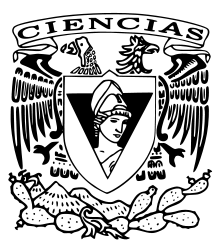
\includegraphics[scale=.29]{img/fciencias1.png}}
	\end{picture}
	
	\begin{center}
		\vspace{-114pt}
		\textbf{\large Matemáticas para las Ciencias II}\\
		\textbf{ Semestre 2020-2}\\
		Prof. Pedro Porras Flores\\
		Ayud. Irving Hernández Rosas \\
		\textbf{Tarea Examen III}\\[0.15cm]
		Kevin Ariel Merino Peña\footnote{Número de cuenta 317031326}\\ [0.12cm]
		\today
	\end{center}
	\vspace{-10pt}
	\rule{19cm}{0.3mm}
	
	\noindent Realice los siguientes ejercicios, escribiendo el procedimiento claramente. Y recuerden la tarea-examen se entregan de manera individual.\\
	
\noindent1.Sea $f: \mathbb{R} \longrightarrow \mathbb{R}$ una función diferenciable. Muestre que $u = f(y - \kappa x)$ es una solución de la ecuación diferencial parcial $$\dfrac{\partial u}{\partial x} + \kappa\dfrac{\partial u}{\partial y} = 0$$
Hagamos una observación sobre $ u $, pues debemos costruir a dicha función con el mismo dominio que f, \textit{i.e. }
\[ u(x,y) = f(y-\kappa x)  \]ahora empleemos la composición de funciones para designar una función auxiliar $ g: \R^2 \to \R $  como sigue $ g(x,y) = y-\kappa x $;
\[ u(x,y) = (f \circ g)(x,y) = f(g(x,y)) \]
luego, tomemos la derivada de $ u $ como 
\[ Du(x,y) = Df(g(x,y)) \]Veamos que, como $ g $ es una función escalar, entonces su derivada es $ \nabla g $ y por la \textbf{regla de la cadena }en funciones compuestas, tenemos que \[ D_u (x,y) = D_f(g(x,y))\nabla g \label{eq:primeraDerivada}\tag{\venus} \]donde $ \nabla g(x,y) = \left( \dfrac{\d g}{\d x}, \dfrac{\d g}{\d y} \right)= \left( -\kappa, 1 \right) $, luego de $ \ref{eq:primeraDerivada} $ tenemos que 
\begin{align*}
	D_u (x,y) &= f'(g(x,y)) \* \left( -\kappa, 1 \right)  && \text{Reemplazando lo que sabemos del gradiente}\\
	D_u (x,y) &= -f'(g(x,y))\kappa, f'(g(x,y)) && \text{Reemplazando lo que sabemos del gradiente}\\
	\dfrac{\d u}{\d x} &= -f'(g(x,y))\kappa  && \text{Derivando con respecto a }x\\
	\dfrac{\d u}{\d y} &= f'(g(x,y)) && \text{Derivando con respecto a }y\\
	\kappa\dfrac{\d u}{\d y} &= f'(g(x,y))\kappa  && \text{Multiplicando ambos miembros por el mismo real }\\
\end{align*}
\[ \dfrac{\partial u}{\partial x} + \kappa\dfrac{\partial u}{\partial y} = -f'(g(x,y))\kappa + f'(g(x,y))\kappa = 0  \]siguiendo la cadena de igualdades, tenemos que 
\[ \dfrac{\partial u}{\partial x} + \kappa\dfrac{\partial u}{\partial y} = 0 \quad \qedsymbol \]

\noindent2.Muestre que si  $u(x,y)$ y $v(x,y)$ tienen segundas parciales mixtas continuas y satisfacen las ecuaciones de 
\begin{subequations}
\label{eq:Maxwell}
Cauchy-Riemann:
\begin{align}
        \dfrac{\partial u}{\partial x} &= \dfrac{\partial v}{\partial y},         \label{eq:MaxB} \\
        \dfrac{\partial u}{\partial y} &= - \dfrac{\partial v}{\partial x}, \label{eq:MaxE}
\end{align}
\end{subequations}

Entonces ambas son armónicas.
\begin{remark}
Una función $u = u(x,y)$ con segundas derivadas parciales continuas que satisface la ecuación de Laplace  $$ \dfrac{\partial^2 u}{\partial x^2} + \dfrac{\partial^2 u}{\partial y^2}= 0,$$ se dice que es una función armónica.
\end{remark}
\noindent Veamos qué ocurre para $ u $ cuando obtenemos sus segundas derivadas
\begin{align*}
	\dfrac{\d^2u}{\d x^2} &= \dfrac{\d}{\d x}\left( \dfrac{\d u}{\d x} \right) &&\text{Por definición de segunda derivada}\\
	\dfrac{\d^2u}{\d x^2} &= \dfrac{\d}{\d x}\left( \dfrac{\d v}{\d x} \right) &&\text{Ya que cumplen las ecuaciones de Cauchy-Riemann}\\
	\dfrac{\d^2u}{\d x^2} &= \dfrac{\d^2 v}{\d x\d y}  &&\text{Volviendo a escribir la ecuación}\\
\end{align*}
por otra parte
\begin{align*}
	\dfrac{\d^2u}{\d y^2} &= \dfrac{\d}{\d y}\left( \dfrac{\d u}{\d y} \right) &&\text{Por definición de segunda derivada}\\
	\dfrac{\d^2u}{\d y^2} &= \dfrac{\d}{\d y}\left( - \dfrac{\d v}{\d x} \right) &&\text{Ya que cumplen las ecuaciones de Cauchy-Riemann}\\
	\dfrac{\d^2u}{\d y^2} &= - \dfrac{\d^2 v}{\d y\d x}&&\text{Reescribiendo}\\
	\dfrac{\d^2u}{\d y^2} &= - \dfrac{\d^2 v}{\d x\d y}&&\text{Ya que por hipótesis $ u $ es de clase }\mathcal{C}^2\\
\end{align*}
de las últimas dos observaciones podemos concluir que
\begin{align*}
	\dfrac{\d^2u}{\d x^2} +\dfrac{\d^2u}{\d y^2} &= \dfrac{\d^2 v}{\d x\d y} +\left( - \dfrac{\d^2 v}{\d x\d y} \right)&&\text{Sumando ambos miembros }\\
	\dfrac{\d^2u}{\d x^2} +\dfrac{\d^2u}{\d y^2} &= 0  &&\text{Así sabemos que $ u $ es armónica}\\
\end{align*}
luego, hagamos algunas observaciones para $ v $

\begin{align*}
\dfrac{\d^2v}{\d x^2} &= \dfrac{\d}{\d x}\left( \dfrac{\d v}{\d x} \right) &&\text{Por definición de segunda derivada}\\
\dfrac{\d^2v}{\d x^2} &= \dfrac{\d}{\d x}\left( - \dfrac{\d u}{\d y} \right) &&\text{Ya que cumplen las ecuaciones de Cauchy-Riemann}\\
\dfrac{\d^2v}{\d x^2} &= - \dfrac{\d^2 u}{\d x\d y}  &&\text{Volviendo a escribir la ecuación}\\
\end{align*}
por otra parte
\begin{align*}
\dfrac{\d^2v}{\d y^2} &= \dfrac{\d}{\d y}\left( \dfrac{\d v}{\d y} \right) &&\text{Por definición de segunda derivada}\\
\dfrac{\d^2v}{\d y^2} &= \dfrac{\d}{\d y}\left(\dfrac{\d u}{\d x} \right) &&\text{Ya que cumplen las ecuaciones de Cauchy-Riemann}\\
\dfrac{\d^2v}{\d y^2} &= \dfrac{\d^2 u}{\d y\d x}&&\text{Reescribiendo}\\
\dfrac{\d^2v}{\d y^2} &=\dfrac{\d^2 u}{\d x\d y}&&\text{Ya que por hipótesis $ v $ es de clase }\mathcal{C}^2\\
\end{align*}
de las últimas dos observaciones podemos concluir que
\begin{align*}
\dfrac{\d^2v}{\d y^2} +\dfrac{\d^2v}{\d x^2} &= \dfrac{\d^2 u}{\d x\d y} +\left( - \dfrac{\d^2 u}{\d x\d y} \right)&&\text{Sumando ambos miembros }\\
\dfrac{\d^2v}{\d y^2} +\dfrac{\d^2v}{\d x^2} &= 0  &&\text{Así sabemos que $ v $ es armónica}\\
\end{align*}
\begin{center}
	$ \therefore $ ambas ecuaciones son armónicas si satisfacen las ecuaciones de  \textit{Cauchy-Riemann} y son de clase $ \mathcal{C}^2 $(que sus segundas derivadas mixtas sean iguales)
\end{center}
\noindent3. Encontrar la expansión a segundo orden de Taylor para $f(x,y) = y^2e^{-x^2}$ en $(1,1)$\\

primero hallemos las derivadas de $ f $
\begin{align*}
	\dfrac{\d}{\d x} \left(y^2 e^{-x^2}\right) &= -2xy^2e^{-x^2} &&\text{Derivando con respecto a }x\\
	\dfrac{\d}{\d y} \left(y^2 e^{-x^2}\right) &= 2ye^{-x^2} &&\text{Derivando con respecto a }y\\
	\dfrac{\d}{\d x} \left(-2xy^2e^{-x^2}\right) &= \left(4x^2 - 2\right)y^2e^{-x^2} &&\text{Derivando con respecto a }xx\\
	\dfrac{\d}{\d y} \left(2y^2e^{-x^2}\right) &= 2e^{-x^2} &&\text{Derivando con respecto a }yy\\
	\dfrac{\d}{\d y} \left(-2xy^2e^{-x^2}\right) &= -4xye^{-x^2} &&\text{Derivando con respecto a }xy, yx\\
\end{align*}
Luego, usando el teorema (visto en clase) sobre la expansión a segundo orden de Taylor para $ x_0 =(1,1) $ está dada por
\begin{align*}
	f(h_1,h_2) &= f(1,1) + h_1f_x(1,1)+ h_2f_y(1,1) + \dfrac{1}{2}\left( h_1^{2}f_{xx}(1,1) + h_1h_2f_{xy}(1,1) + h_1h_2f_{yx}(1,1) + h_2^2f_{yy}(1,1) \right)\\
	f(x,y) &= f(1,1) + xf_x(1,1)+ yf_y(1,1) + \dfrac{1}{2}\left( h_1^2f_{xx}(1,1) + h_1h_2f_{xy}(1,1) + h_1h_2f_{yx}(1,1) + h_2^2f_{yy}(1,1) \right)\\
	f(x,y) &= f(1,1) + x\dfrac{\d f}{\d x}\Bigr|_{(1,1)}+ y\dfrac{\d f}{\d y}\Bigr|_{(1,1)} + \dfrac{1}{2}\left( h_1^2\dfrac{\d^2 f}{\d x^2}\Bigr|_{(1,1)} + h_1h_2\dfrac{\d^2 f}{\d x \d y}\Bigr|_{(1,1)} + h_1h_2\dfrac{\d^2 f}{\d y \d x}\Bigr|_{(1,1)}+ h_2^2\dfrac{\d^2 f}{\d y^2 }\Bigr|_{(1,1)}\right)\\
	f(x,y) &= 1^2e^{-1^2} + x\left( -2xy^2e^{-x^2} \right)\Bigr|_{(1,1)}+ y\dfrac{\d f}{\d y}\Bigr|_{(1,1)} + \dfrac{1}{2}\left( h_1^2\dfrac{\d^2 f}{\d x^2}\Bigr|_{(1,1)} + h_1h_2\dfrac{\d^2 f}{\d x \d y}\Bigr|_{(1,1)} + h_1h_2\dfrac{\d^2 f}{\d y \d x}\Bigr|_{(1,1)}+ h_2^2\dfrac{\d^2 f}{\d y^2 }\Bigr|_{(1,1)}\right)\\
	f(x,y) &= \dfrac{1}{e} -\dfrac{2h_1}{e} + \dfrac{2h_2}{e} + \dfrac{1}{2}\left( h_1^2\dfrac{\d^2 f}{\d x^2}\Bigr|_{(1,1)} + h_1h_2\dfrac{\d^2 f}{\d x \d y}\Bigr|_{(1,1)} + h_1h_2\dfrac{\d^2 f}{\d y \d x}\Bigr|_{(1,1)}+ h_2^2\dfrac{\d^2 f}{\d y^2 }\Bigr|_{(1,1)}\right)\\
	f(x,y) &= \dfrac{1}{e} -\dfrac{2h_1}{e} + \dfrac{2h_2}{e} + \dfrac{1}{2}\left( h_1^2(2e^{-1}) + h_1h_2(-4e^{-1}) + h_1h_2(-4e^{-1}) + h_2^2(2e^{-1})  \right)\\
	f(x,y) &= \dfrac{1}{e} -\dfrac{2h_1}{e} + \dfrac{2h_2}{e} + \dfrac{h_1^2  -4h_1h_2 + h_2^2}{e}\\
	f(x,y) &=  \dfrac{x^2-4xy+y^2+4y-1}{e}\\
\end{align*}

\noindent4. Sea $f: \mathbb{R}^2 \longrightarrow \mathbb{R}$ tal que  $f(x,y) = x^2 - y^2 - xy + 5$. Encuentre los puntos críticos de $f$ y determine si son: mínimos locales, máximos locales o puntos silla.\\
Para ello derivemos la función y localicemos los puntos críticos.

\begin{align*}
	\dfrac{\d f}{\d x} &= \dfrac{\d }{\d x}\left( x^2 - y^2 - xy + 5 \right) &&\text{Derivando con respecto a }x\\
	\dfrac{\d f}{\d x} &= 2x-y &&\text{Aplicando la derivada}\\
	\dfrac{\d f}{\d x} &= -2y-x &&\text{Aplicando la derivada con respecto a $ y $ de }f\\
	\\
	0 &= 2x-y &&\text{Igualemos a }0\\
	0 &= -2y - x &&\text{ }\\
\end{align*}
De la primera ecuación, obtenemos que $ y = 2x $, sustituyendo en la segunda ecuación obtenemos que $ 0 = -5x $, de esta manera sabemos que el único punto crítico que tiene $ f $ es $ (x,y) = (0,0) $. Ahora calculemos las segundas derivadas parciales para conocer el determinante del Hessiano
\begin{align*}
	\dfrac{\d^2 f}{\d x^2} &= 2\\
	\dfrac{\d^2 f}{\d y^2} &= -2\\
	\dfrac{\d^2 f}{\d y \d x} &= -1\\
	\dfrac{\d^2 f}{\d x \d y} &= -1\\
	D\Bigr|_{(0,0)} &= 2 \* (-2) - 1 = -5 < 0\\
\end{align*}
Entonces, usando el teorema visto en clase sobre el determinante del hessiano, ahora sabemos que $ (0,0) $ es un punto silla, es más es el único punto crítico de $ f $.\\


\noindent5. Encuentre los valores máximos y mínimos absolutos de $f(x,y) = x^2 + 3xy + y^2 + 5$ sobre el disco unitario $\mathcal{D} = \{(x,y) \in \mathbb{R}^2 : x^2 + y^2 \leq 1 \}$\\

\noindent6. Suponga que un pentágono está compuesto por un rectángulo coronado por un triángulo isósceles (ver Figura \ref{fig:1}). Si la longitud del perímetro es fija, encuentre el área máxima posible.

\begin{figure}[h]
    \centering
    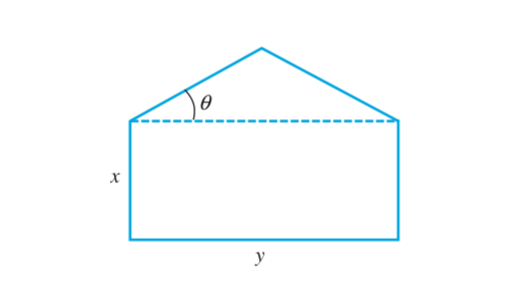
\includegraphics[width=0.5\textwidth]{img/figT}
    \caption{Maximizar el área para un perímetro dado.}
    \label{fig:1}
\end{figure}


\noindent7. Analice el comportamiento de las funciones en los puntos indicados. En la parte $b$ el análisis depende de la constante $C$.\\


a) $z = x^2 - y^2 + 3xy $ en $(0,0)$.\\
b)  $z = x^2 - y^2 + Cxy $ en $(0,0)$.




\noindent8. a) Encuentre la distancia mínima del origen en $\mathbb{R}^2$  a la superficie $z = \sqrt{x^2 - 1}$.\\

b) Haga lo mismo para la superficie $z = 6xy + 7$\\

\noindent9. Encuentre los puntos y valores críticos de las siguientes funciones sujetas a las restricciones:\\


a) $f(x,y) = x^2 - 2xy + 2y^2$, restringido a $x^2 + y^2 =1$.\\

b) $f(x,y) = \cos{(x^2 - y^2)}{}$, restringido a $x^2 + y^2 =1$.\\

c) $f(x,y) = \dfrac{x^2 - y^2}{x^2 + y^2}$, restringido a $x + y =1$.\\

d) $f(x,y) = \cos^2{x} +\cos^2{y}$, restringido a $x + y =\frac{\pi}{4}$.


\noindent10. Encuentre el máximo de la función $f(x,y) = xy$ sobre la curva $(x +1)^2 + y^2 =1$

\noindent11. Encuentre la distancia más cercana del punto $(a_1, a_2, a_3) \in \mathbb{R}^3$ al plano cuya ecuación está dada por: $b_1x_1 + b_2x_2 + b_3x_3 + b_0 = 0$, donde $(b_1, b_2, b_3) \neq 0 $

\noindent12. Encuentre el punto sobre la linea de intersección de los planos  $a_1x_1 + a_2x_2 + a_3x_3 = 0$ y $b_1x_1 + b_2x_2 + b_3x_3 + b_0 = 0$ que es más cercano al origen.

\end{document}
